\documentclass{article}
\usepackage{amsmath} %This allows me to use the align functionality.
                   %If you find yourself trying to replicate
                   %something you found online, ensure you're
                   %loading the necessary packages!
\usepackage{amsfonts}%Math font
\usepackage{graphicx}%For including graphics
\usepackage{hyperref}%For Hyperlinks
\usepackage{natbib}        %For the bibliography
\bibliographystyle{apalike}%For the bibliography
\usepackage[margin=1.0in]{geometry}
\usepackage{float}
\usepackage{Sweave}
\begin{document}
\Sconcordance{concordance:HW4.tex:HW4.Rnw:%
1 12 1 1 0 30 1 1 3 6 0 1 3 1 2 7 0 1 1 7 0 2 2 1 0 2 1 1 5 8 0 2 2 6 0 %
1 1 5 0 1 1 6 0 1 2 29 1 1 2 1 0 2 1 19 0 1 2 1 1 1 2 1 0 1 6 9 0 2 2 1 %
0 3 1 12 0 1 1 12 0 1 1 22 0 1 2 29 1 1 2 1 0 3 1 3 0 2 2 1 0 1 1 21 0 %
1 1 6 0 1 2 1 1 1 2 1 0 2 1 3 0 2 2 1 0 1 1 22 0 1 2 2 1 1 3 2 0 1 8 7 %
0 1 2 1 7 6 0 1 2 4 0 2 2 7 0 1 2 1 4 3 0 1 6 9 0 1 2 3 1 1 2 1 0 2 1 3 %
0 2 2 1 0 1 1 22 0 1 2 2 1 1 3 2 0 1 8 7 0 1 2 1 7 6 0 1 2 4 0 2 2 7 0 %
1 2 1 4 3 0 1 6 9 0 1 2 2 1 1 3 2 0 3 1 3 0 2 2 1 0 1 1 22 0 1 2 3 1 1 %
3 2 0 1 8 7 0 1 2 1 7 6 0 1 2 4 0 2 2 7 0 1 2 1 4 3 0 1 6 9 0 1 2 10 1 %
1 2 1 0 3 1 3 0 2 2 4 0 1 2 14 1 1 2 1 0 1 1 3 0 1 2 77 1 1 3 2 0 1 1 3 %
0 1 2 2 1 1 2 1 0 1 1 34 0 1 2 1 3 2 0 1 1 32 0 1 1 6 0 1 2 8 1}

%set the size of the graphs to fit nicely on a 8.5x11 sheet
\noindent \textbf{MA 354: Data Analysis I -- Fall 2019}\\%\\ gives you a new line
\noindent \textbf{Homework 3:}\vspace{1em}\\
\emph{Complete the following opportunities to use what we've talked about in class. 
These questions will be graded for correctness, communication and succinctness. Ensure
you show your work and explain your logic in a legible and refined submission.}\\
%Comments -- anything after % is not put into the PDF

\begin{enumerate}
%%%%%%%%%%%%%%%%%%%%%%%%%%%%%%%%%%%%%%%%%%%%%%%%%%%%%%%%%%%%%%%%%%%%%%%%%%%%%%%
%%%%%%%%%%%%%%%%%%%%%%%%%%%%%%%%%%%%%%%%%%%%%%%%%%%%%%%%%%%%%%%%%%%%%%%%%%%%%%%
%%%%%%%%%  Question 0
%%%%%%%%%%%%%%%%%%%%%%%%%%%%%%%%%%%%%%%%%%%%%%%%%%%%%%%%%%%%%%%%%%%%%%%%%%%%%%%
%%%%%%%%%%%%%%%%%%%%%%%%%%%%%%%%%%%%%%%%%%%%%%%%%%%%%%%%%%%%%%%%%%%%%%%%%%%%%%%
\item[0.] \textbf{Complete weekly diagnostics.}

%%%%%%%%%%%%%%%%%%%%%%%%%%%%%%%%%%%%%%%%%%%%%%%%%%%%%%%%%%%%%%%%%%%%%%%%%%%%%%%
%%%%%%%%%%%%%%%%%%%%%%%%%%%%%%%%%%%%%%%%%%%%%%%%%%%%%%%%%%%%%%%%%%%%%%%%%%%%%%%
%%%%%%%%%  Question 1
%%%%%%%%%%%%%%%%%%%%%%%%%%%%%%%%%%%%%%%%%%%%%%%%%%%%%%%%%%%%%%%%%%%%%%%%%%%%%%%
%%%%%%%%%%%%%%%%%%%%%%%%%%%%%%%%%%%%%%%%%%%%%%%%%%%%%%%%%%%%%%%%%%%%%%%%%%%%%%%
\item  	Plankton samples are typically collected using fine mesh nets towed from research vessels, and larval fish are removed then stored after sample preservation. Samples are frequently collected using the paired bongo net, which consists of two usually round net frames joined at a central point, and towed either obliquely or vertically through the water column. Mesopelagic fish families such as the Myctophidae are some of the most specious and abundant in the worlds oceans. We expect the number of Myctophidae in the left and right side of each net to be highly correlated, but we want to quantify this relationship. 
	
	\cite{Muhling} provide data on a total of 261 paired samples from the Gulf of Mexico. Myctophidae counts from the left and right sides of each bongo net are a result of over years (1987-2008) of sampling. We define $X$ and $Y$ to be the count of myctophid larvae in the left and right side of the bongo net, respectively.
	
\textbf{Research Question:} Does the data we have confirm our expectation that the number of Myctophidae in the left and right side of each net tend to be highly correlated? 

The data can be loaded as follows. The data for the number of fish caught in the left and
right net are in the columns labeled \texttt{Left} and \texttt{Right}, respectively.
\begin{Schunk}
\begin{Sinput}
> dat.bongo<-read.csv(file = "https://cipolli.com/students/data/BongoNetData.txt",
+                       header = TRUE,sep = ",")
> 
\end{Sinput}
\end{Schunk}

\begin{Schunk}
\begin{Sinput}
> summary(dat.bongo$Left)
\end{Sinput}
\begin{Soutput}
   Min. 1st Qu.  Median    Mean 3rd Qu.    Max. 
   1.00   14.00   27.00   42.09   53.00  303.00 
\end{Soutput}
\begin{Sinput}
> summary(dat.bongo$Right)
\end{Sinput}
\begin{Soutput}
   Min. 1st Qu.  Median    Mean 3rd Qu.    Max. 
   1.00   18.00   33.00   50.07   66.00  300.00 
\end{Soutput}
\end{Schunk}

\begin{Schunk}
\begin{Sinput}
> library(ggplot2)
> library(gridExtra)
> ggdat<-data.frame(left=dat.bongo$Left, right=dat.bongo$Right)
> ggplot(data=ggdat,aes(x = right, y= left))+
+   geom_point()+
+   geom_smooth(alpha=0.25,color="black",method="loess")+
+   theme_bw()+
+   ggtitle("Left and Right Sides of a Bongo Net")
\end{Sinput}
\end{Schunk}
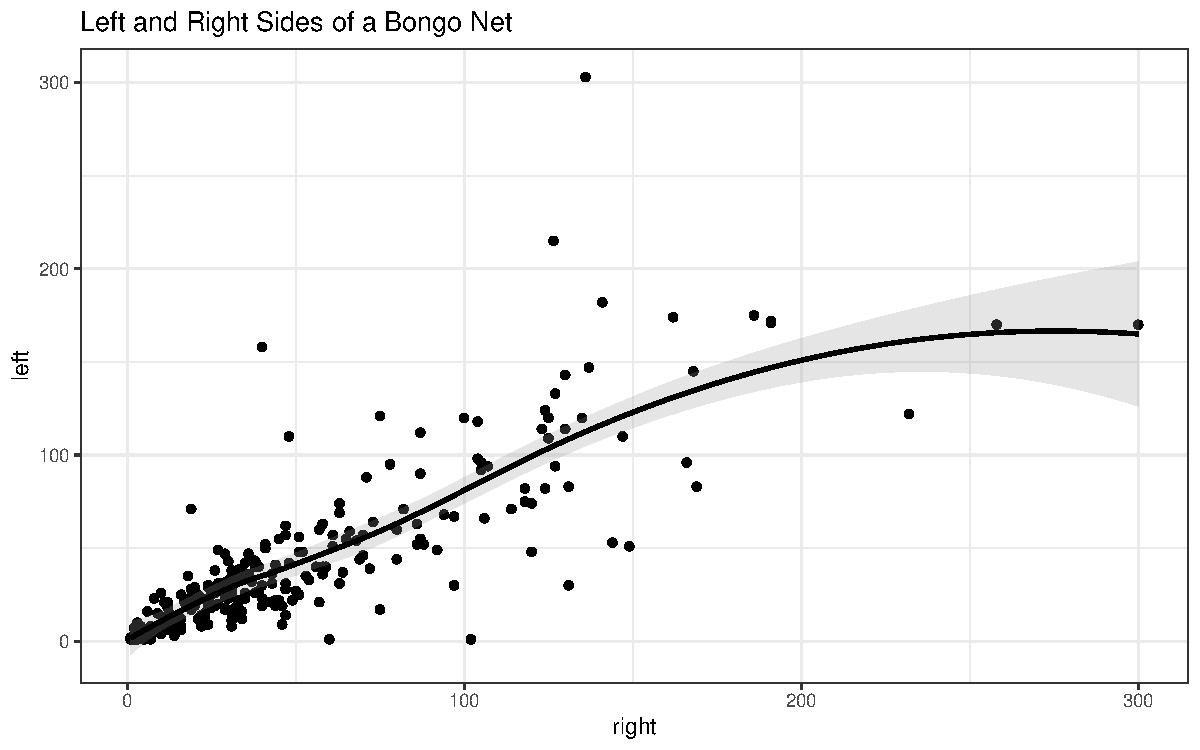
\includegraphics{HW4-003}

\begin{Schunk}
\begin{Sinput}
> cor(dat.bongo$Left,dat.bongo$Right,method = "pearson")
\end{Sinput}
\begin{Soutput}
[1] 0.8232054
\end{Soutput}
\begin{Sinput}
> cor(dat.bongo$Left,dat.bongo$Right,method = "kendall")
\end{Sinput}
\begin{Soutput}
[1] 0.7105615
\end{Soutput}
\begin{Sinput}
> cor(dat.bongo$Left,dat.bongo$Right,method = "spearman")
\end{Sinput}
\begin{Soutput}
[1] 0.8639953
\end{Soutput}
\end{Schunk}

**Would we want to use a kendall or a spearman's rank because the graph shows that the correlation isn't totally linear?

%%%%%%%%%%%%%%%%%%%%%%%%%%%%%%%%%%%%%%%%%%%%%%%%%%%%%%%%%%%%%%%%%%%%%%%%%%%%%%%
%%%%%%%%%%%%%%%%%%%%%%%%%%%%%%%%%%%%%%%%%%%%%%%%%%%%%%%%%%%%%%%%%%%%%%%%%%%%%%%
%%%%%%%%%  Question 2
%%%%%%%%%%%%%%%%%%%%%%%%%%%%%%%%%%%%%%%%%%%%%%%%%%%%%%%%%%%%%%%%%%%%%%%%%%%%%%%
%%%%%%%%%%%%%%%%%%%%%%%%%%%%%%%%%%%%%%%%%%%%%%%%%%%%%%%%%%%%%%%%%%%%%%%%%%%%%%%
\item \textbf{(Working with Data)} Hepatitis C is a disease 
    that affects the liver. The virus that causes hepatitis C 
    is spread through blood or bodily fluids of an infected person. 
    The virus is often difficult to diagnose because there are few unique 
    symptoms. Those infected, however, sometimes experience jaundice -- a 
    condition that causes yellowing of the skin or eyes, as the liver 
    is infected.

    \cite{Bracht16} consider the human microfibrillar-associated protein 4,
    or MFAP4, and its role in disease-related tissue. Stage 0--no fibrosis; 
    Stage 1--enlarged, fibrotic portal tracts; Stage 2--periportal fibrosis 
    or portal-portal septa, but intact architecture; Stage 3--fibrosis with
    architectural distortion, but no obvious cirrhosis; and Stage 4--probable
    or definite cirrhosis.

    Previously, it has been shown that MFAP4 is a biomarker candidate for hepatic
    fibrosis and cirrhosis in hepatitis C patients. The analysis of \cite{Bracht16}
    aimed to consider the ability of MFAP4 to differentiate between stages of the 
    disease -- fibrosis stages (0-2) and cirrhosis (3-4) based on the Scheuer 
    scoring system.
    
    Below, I load the data from the web.
\begin{Schunk}
\begin{Sinput}
> fn<-"http://cipolli.com/students/data/biomarker.csv"
> dat <- read.csv(file=fn, header=TRUE, sep=",")
> head(dat)
\end{Sinput}
\begin{Soutput}
  Patient.ID Year.of.Birth Gender Date.of.sampling Fibrosis.Stage HCV.Genotype
1       1112          1958 female         2/1/2005              0            1
2       3403          1946 female        1/18/2005              2             
3       2841          1954 female         1/3/2005              3            1
4        654          1958   male         2/1/2005              3            1
5       2788          1960   male        12/9/2004              0            3
6       2242          1954 female        5/12/2004              0            1
  MFAP4.U.mL
1        5.1
2        5.3
3       12.9
4        6.2
5        3.3
6        7.5
\end{Soutput}
\end{Schunk}
In homework 0, you recreated Table 1 in \href{the paper}{https://www.ncbi.nlm.nih.gov/pmc/articles/PMC4932744/}. 
Now, recreate Table 2.
\begin{Schunk}
\begin{Sinput}
> ggdat<-data.frame(fibrosis=dat$Fibrosis.Stage, MFAP4=dat$MFAP4.U.mL)
> ggplot(data=ggdat,aes(x=fibrosis, y=MFAP4, group=fibrosis))+
+   geom_violin(fill="lightblue")+
+   geom_boxplot(width=0.25)+
+   theme_bw()+
+   xlab("Fibrosis Stage")+
+   ylab("MFAP4")
\end{Sinput}
\end{Schunk}
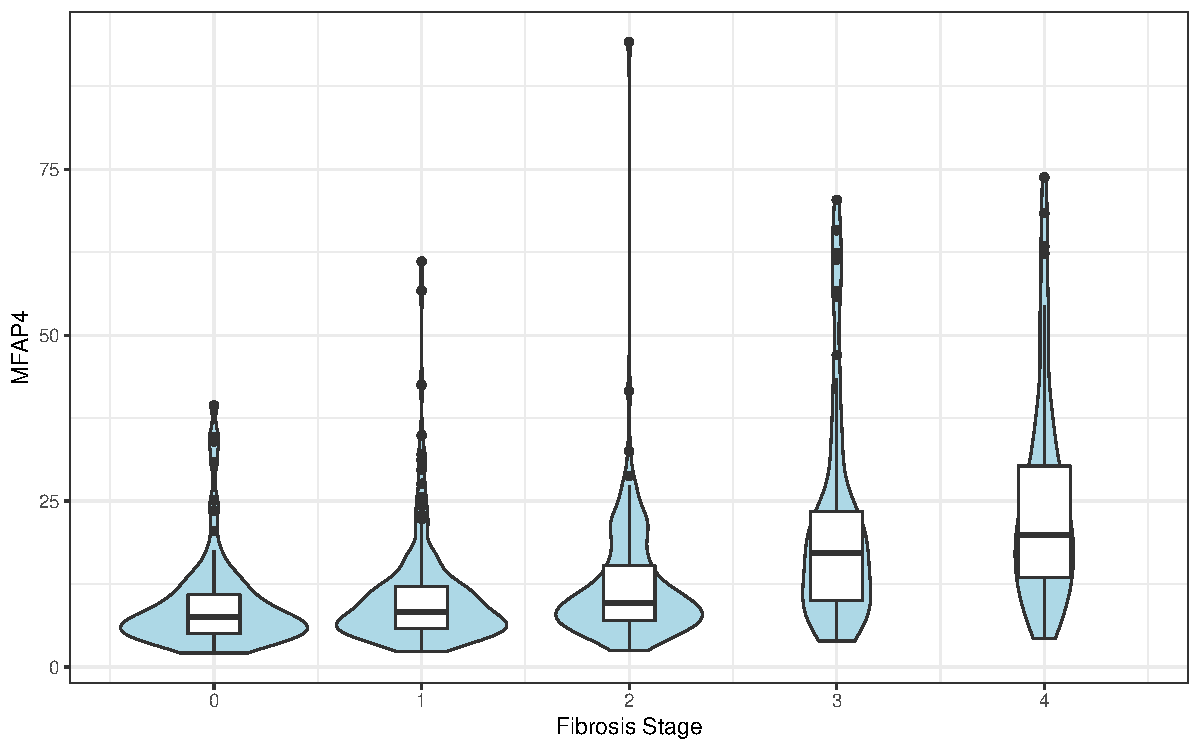
\includegraphics{HW4-006}

\begin{Schunk}
\begin{Sinput}
> dat.f<-ggdat
> dat.f$fibrosis<-as.factor(dat.f$fibrosis)
> dat.f$MFAP4<-as.factor(dat.f$MFAP4)
> anova(lm(dat$MFAP4.U.mL~dat$Fibrosis.Stage))
\end{Sinput}
\begin{Soutput}
Analysis of Variance Table

Response: dat$MFAP4.U.mL
                    Df Sum Sq Mean Sq F value    Pr(>F)    
dat$Fibrosis.Stage   1  13584 13583.9  112.67 < 2.2e-16 ***
Residuals          540  65102   120.6                      
---
Signif. codes:  0 ‘***’ 0.001 ‘**’ 0.01 ‘*’ 0.05 ‘.’ 0.1 ‘ ’ 1
\end{Soutput}
\begin{Sinput}
> anova(lm(MFAP4.U.mL~Fibrosis.Stage, data=dat))
\end{Sinput}
\begin{Soutput}
Analysis of Variance Table

Response: MFAP4.U.mL
                Df Sum Sq Mean Sq F value    Pr(>F)    
Fibrosis.Stage   1  13584 13583.9  112.67 < 2.2e-16 ***
Residuals      540  65102   120.6                      
---
Signif. codes:  0 ‘***’ 0.001 ‘**’ 0.01 ‘*’ 0.05 ‘.’ 0.1 ‘ ’ 1
\end{Soutput}
\begin{Sinput}
> TukeyHSD(aov(lm(dat$MFAP4.U.mL~as.factor(dat$Fibrosis.Stage)), conf.level = 0.95))
\end{Sinput}
\begin{Soutput}
  Tukey multiple comparisons of means
    95% family-wise confidence level

Fit: aov(formula = lm(dat$MFAP4.U.mL ~ as.factor(dat$Fibrosis.Stage)), conf.level = 0.95)

$`as.factor(dat$Fibrosis.Stage)`
         diff        lwr       upr     p adj
1-0  1.301353 -2.4541799  5.056886 0.8777020
2-0  3.153807 -0.7991649  7.106778 0.1874077
3-0 11.741745  7.0240362 16.459454 0.0000000
4-0 15.388014 10.6703049 20.105722 0.0000000
2-1  1.852454 -1.5452808  5.250188 0.5679669
3-1 10.440392  6.1771314 14.703652 0.0000000
4-1 14.086660  9.8234000 18.349921 0.0000000
3-2  8.587938  4.1497688 13.026107 0.0000017
4-2 12.234207  7.7960375 16.672376 0.0000000
4-3  3.646269 -1.4848264  8.777364 0.2948449
\end{Soutput}
\end{Schunk}
    \begin{table}[H]
  \centering
    \begin{tabular}{lccccc}\hline
    Comparison & Difference & Lower Bound & Upper Bound & $p$ value\\\hline\hline
    F1-F0                   &  &   &   &\\
    F2-F0                   &  &   &   &\\
    F3-F0                   &  &   &   &\\
    F4-F0                   &  &   &   &\\
    F2-F1                   &  &   &   &\\
    F3-F1                   &  &   &   &\\
    F4-F1                   &  &   &   &\\
    F3-F2                   &  &   &   &\\
    F4-F2                   &  &   &   &\\
    F4-F3                   &  &   &   &\\\hline
    \end{tabular}
    \caption{Results of the pairwise comparisons of individual
    hepatic fibrosis stages with  respect to MFAP4 values
    after significant ANOVA result.} \label{MFAP4.ANOVA}
  \end{table}
** Are the results I get different from the table because the table uses log MFAP4 values?
%%%%%%%%%%%%%%%%%%%%%%%%%%%%%%%%%%%%%%%%%%%%%%%%%%%%%%%%%%%%%%%%%%%%%%%%%%%%%%%
%%%%%%%%%%%%%%%%%%%%%%%%%%%%%%%%%%%%%%%%%%%%%%%%%%%%%%%%%%%%%%%%%%%%%%%%%%%%%%%
%%%%%%%%%  Question 3
%%%%%%%%%%%%%%%%%%%%%%%%%%%%%%%%%%%%%%%%%%%%%%%%%%%%%%%%%%%%%%%%%%%%%%%%%%%%%%%
%%%%%%%%%%%%%%%%%%%%%%%%%%%%%%%%%%%%%%%%%%%%%%%%%%%%%%%%%%%%%%%%%%%%%%%%%%%%%%%
  \item Complete the following parts. This will lead you through the simulation
  of data, fitting regression lines and evaluating the assumptions.
  \begin{enumerate}
  \item Fit a model to the following simulated data. Make observations about
  the model equation and the Pearson correlation.
\begin{Schunk}
\begin{Sinput}
> n=500
> x<-sample(x = seq(0,5,0.01),size = n,replace = T)
> y<-5*x + 3
> plot(x,y)
\end{Sinput}
\end{Schunk}

\begin{Schunk}
\begin{Sinput}
> xy.mod<-lm(y~x) 
> summary(xy.mod) 
\end{Sinput}
\begin{Soutput}
Call:
lm(formula = y ~ x)

Residuals:
       Min         1Q     Median         3Q        Max 
-8.804e-14 -5.590e-16  1.810e-16  8.800e-16  3.788e-15 

Coefficients:
             Estimate Std. Error   t value Pr(>|t|)    
(Intercept) 3.000e+00  3.831e-16 7.831e+15   <2e-16 ***
x           5.000e+00  1.308e-16 3.822e+16   <2e-16 ***
---
Signif. codes:  0 ‘***’ 0.001 ‘**’ 0.01 ‘*’ 0.05 ‘.’ 0.1 ‘ ’ 1

Residual standard error: 4.238e-15 on 498 degrees of freedom
Multiple R-squared:      1,	Adjusted R-squared:      1 
F-statistic: 1.461e+33 on 1 and 498 DF,  p-value: < 2.2e-16
\end{Soutput}
\begin{Sinput}
> cor(x,y, method = "pearson") #is the R squared the pearson correlation?
\end{Sinput}
\begin{Soutput}
[1] 1
\end{Soutput}
\end{Schunk}
  \item Fit a model to the following simulated data, now with added Normal error. Make
  observations about the model equation and the Pearson correlation in relation to (a).
\begin{Schunk}
\begin{Sinput}
> e<-rnorm(n=n,mean=0,sd=3)
> y2<-5*x + 3 + e
> plot(x,y2)
\end{Sinput}
\end{Schunk}

\begin{Schunk}
\begin{Sinput}
> xy2.mod<-lm(y2~x)
> summary(xy2.mod)
\end{Sinput}
\begin{Soutput}
Call:
lm(formula = y2 ~ x)

Residuals:
    Min      1Q  Median      3Q     Max 
-9.3521 -1.8736  0.1815  2.0200  8.4481 

Coefficients:
            Estimate Std. Error t value Pr(>|t|)    
(Intercept)  2.88840    0.27288   10.59   <2e-16 ***
x            5.11015    0.09319   54.84   <2e-16 ***
---
Signif. codes:  0 ‘***’ 0.001 ‘**’ 0.01 ‘*’ 0.05 ‘.’ 0.1 ‘ ’ 1

Residual standard error: 3.019 on 498 degrees of freedom
Multiple R-squared:  0.8579,	Adjusted R-squared:  0.8576 
F-statistic:  3007 on 1 and 498 DF,  p-value: < 2.2e-16
\end{Soutput}
\end{Schunk}
  \item In the model of part (b), test for normality and constance of error terms. Note 
  that we know both of these items to be true since we've taken $\epsilon \sim 
  \textrm{N}(\mu=0,\sigma=3)$.
\begin{Schunk}
\begin{Sinput}
> #check for normality - plots residuals
> ggdat<-data.frame(residuals=xy2.mod$residuals)
> g1<-ggplot(data=ggdat,aes(x=residuals))+
+   geom_histogram(aes(y=..density..),
+                  fill="lightblue",color="black",bins=8)+
+   geom_hline(yintercept=0)+
+   geom_density(fill="red", alpha = 0.2)+
+   theme_bw()+
+   xlab("Residuals")+
+   ylab("Density")
> library("qqplotr")
> g2<-ggplot(data=ggdat,aes(sample=residuals))+
+   stat_qq_band(alpha=0.25) +
+   stat_qq_line() +
+   stat_qq_point() +
+   theme_bw()+
+   xlab("Gaussian Quantiles")+
+   ylab("Sample Quantiles")
> grid.arrange(g1,g2,ncol=2)
\end{Sinput}
\end{Schunk}
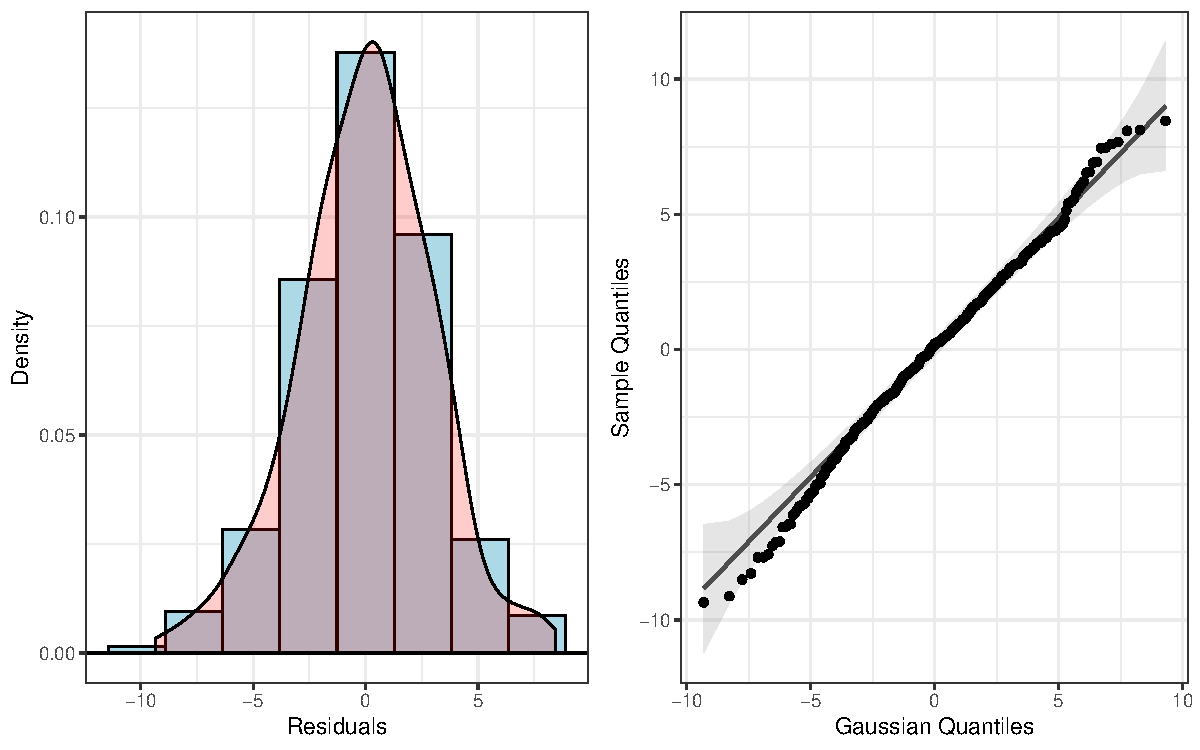
\includegraphics{HW4-012}

\begin{Schunk}
\begin{Sinput}
> sum(xy2.mod$residuals) #close to zero
\end{Sinput}
\begin{Soutput}
[1] 8.312795e-15
\end{Soutput}
\end{Schunk}

\begin{Schunk}
\begin{Sinput}
> #check constance - plot residuals against fitted values
> ggdat<-data.frame(residuals=xy2.mod$residuals,
+                   fitted=xy2.mod$fitted.values)
> ggplot(data=ggdat, aes(x=fitted, y=residuals))+
+   geom_point(shape=1) +
+   geom_hline(yintercept=0, linetype="dashed")+
+   theme_bw()+
+   xlab(bquote(hat(Y)))+
+   ylab("Residuals")
\end{Sinput}
\end{Schunk}
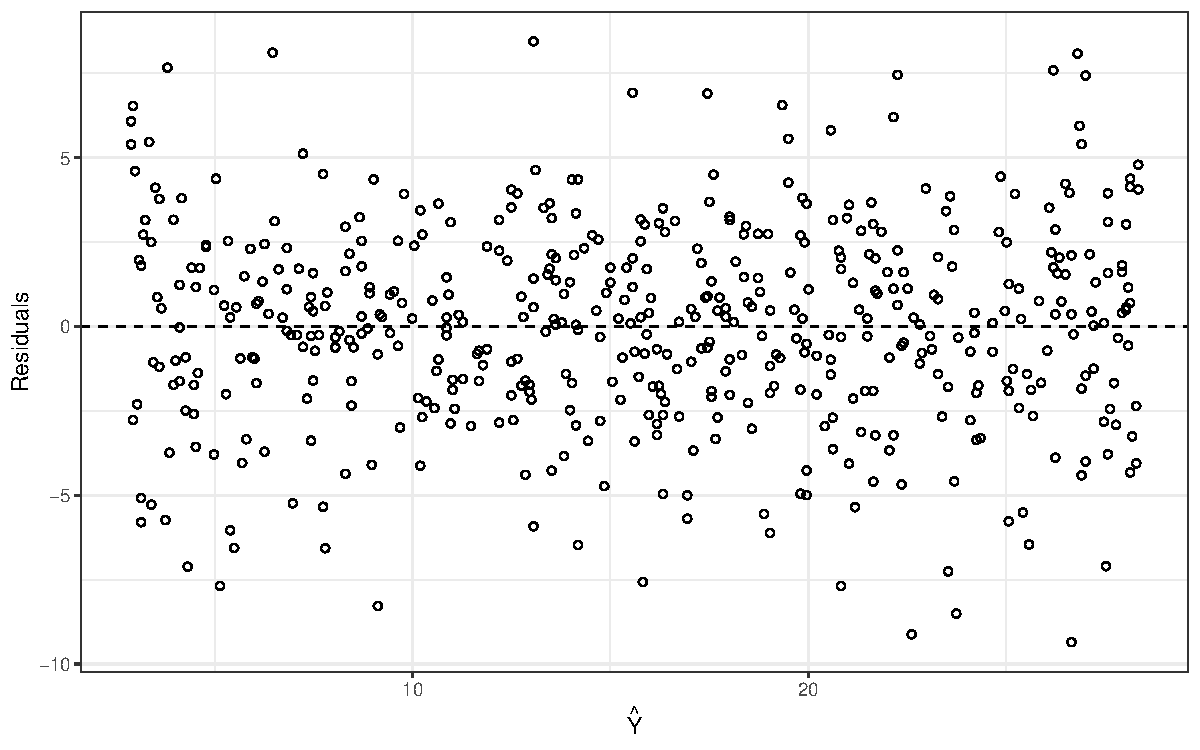
\includegraphics{HW4-014}

  \item Fit a model to the following simulated data, now with added exponential error.
  Make observations about the model equation and the Pearson correlation in relation 
  to the model of part (b).
\begin{Schunk}
\begin{Sinput}
> e<-rexp(n=n,rate = 1/2)
> y3<-5*x + 3 + e
> plot(x,y3)
\end{Sinput}
\end{Schunk}

\begin{Schunk}
\begin{Sinput}
> xy3.mod<-lm(y3~x)
> summary(xy3.mod)
\end{Sinput}
\begin{Soutput}
Call:
lm(formula = y3 ~ x)

Residuals:
    Min      1Q  Median      3Q     Max 
-2.2405 -1.4410 -0.7256  0.9924  8.5343 

Coefficients:
            Estimate Std. Error t value Pr(>|t|)    
(Intercept)  5.26540    0.18206   28.92   <2e-16 ***
x            4.93482    0.06217   79.37   <2e-16 ***
---
Signif. codes:  0 ‘***’ 0.001 ‘**’ 0.01 ‘*’ 0.05 ‘.’ 0.1 ‘ ’ 1

Residual standard error: 2.014 on 498 degrees of freedom
Multiple R-squared:  0.9267,	Adjusted R-squared:  0.9266 
F-statistic:  6300 on 1 and 498 DF,  p-value: < 2.2e-16
\end{Soutput}
\end{Schunk}
  \item In the model of part (d), test for normality and constance of error terms. Note
  that we know that common variance is true but we've taken $\epsilon \sim 
  \textrm{exp}(\beta=2)$.
\begin{Schunk}
\begin{Sinput}
> #check for normality - plots residuals
> ggdat<-data.frame(residuals=xy3.mod$residuals)
> g1<-ggplot(data=ggdat,aes(x=residuals))+
+   geom_histogram(aes(y=..density..),
+                  fill="lightblue",color="black",bins=8)+
+   geom_hline(yintercept=0)+
+   geom_density(fill="red", alpha = 0.2)+
+   theme_bw()+
+   xlab("Residuals")+
+   ylab("Density")
> library("qqplotr")
> g2<-ggplot(data=ggdat,aes(sample=residuals))+
+   stat_qq_band(alpha=0.25) +
+   stat_qq_line() +
+   stat_qq_point() +
+   theme_bw()+
+   xlab("Gaussian Quantiles")+
+   ylab("Sample Quantiles")
> grid.arrange(g1,g2,ncol=2)
\end{Sinput}
\end{Schunk}
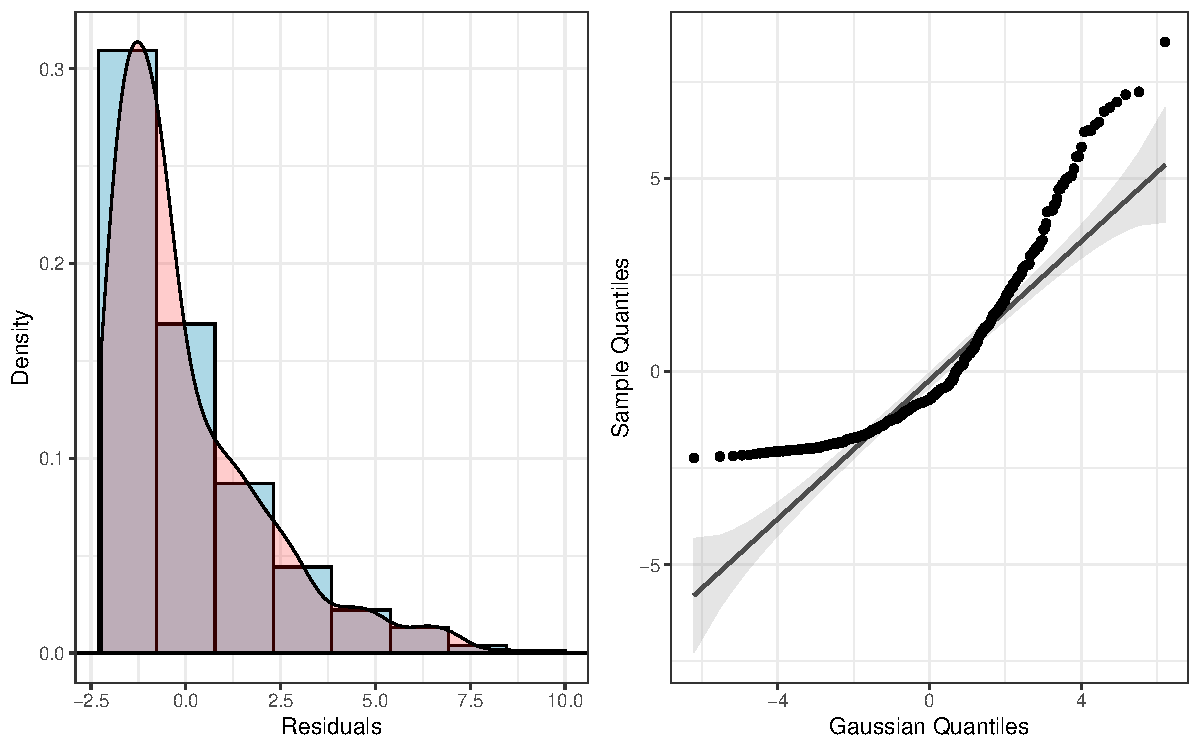
\includegraphics{HW4-017}

\begin{Schunk}
\begin{Sinput}
> sum(xy3.mod$residuals) #close to zero
\end{Sinput}
\begin{Soutput}
[1] -4.96686e-14
\end{Soutput}
\end{Schunk}

\begin{Schunk}
\begin{Sinput}
> #check constance - plot residuals against fitted values
> ggdat<-data.frame(residuals=xy3.mod$residuals,
+                   fitted=xy3.mod$fitted.values)
> ggplot(data=ggdat, aes(x=fitted, y=residuals))+
+   geom_point(shape=1) +
+   geom_hline(yintercept=0, linetype="dashed")+
+   theme_bw()+
+   xlab(bquote(hat(Y)))+
+   ylab("Residuals")
\end{Sinput}
\end{Schunk}
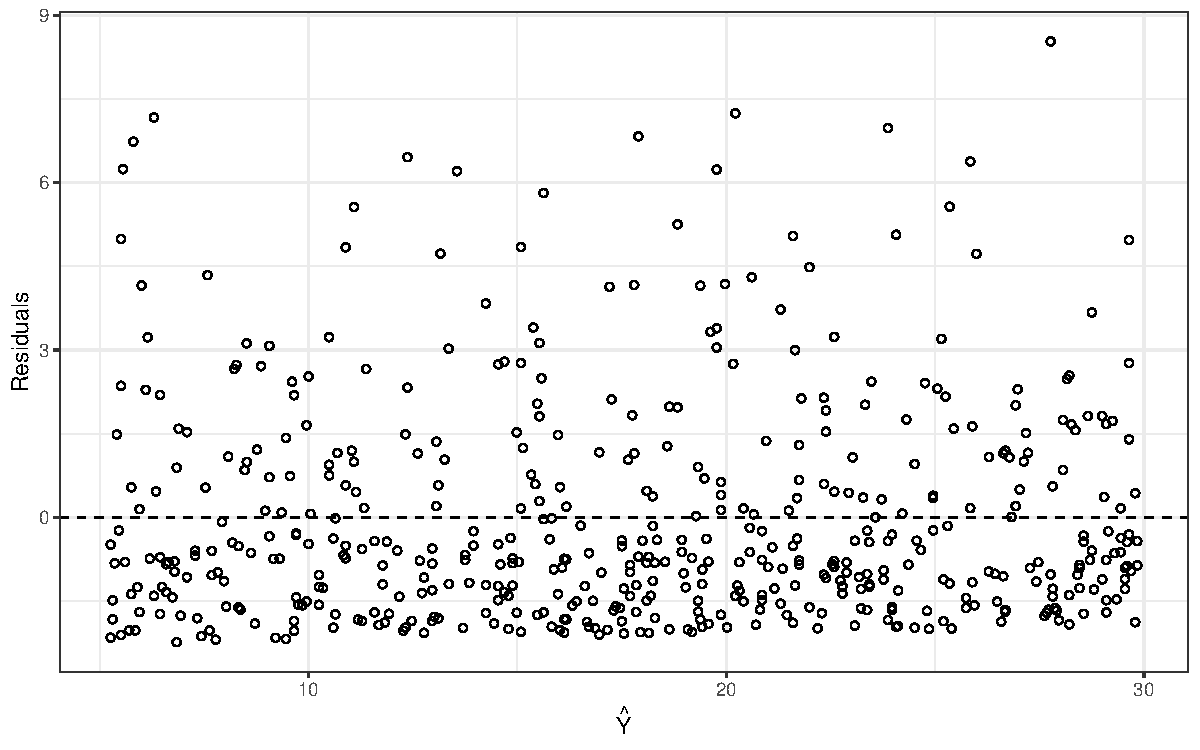
\includegraphics{HW4-019}
  \item Fit a model to the following simulated data, now with added Heteroskedastic
  normal error. Make observations about the model equation and the Pearson correlation
  in relation to the model of part (b).
\begin{Schunk}
\begin{Sinput}
> #order X to simulate non constant error
> x4<-x[order(x)]
> e<-rnorm(n=n,mean=0,sd=c(rep(1,n/2),rep(3,n/2)))
> y4<-5*x4 + 3 + e
> plot(x4,log(y4))
\end{Sinput}
\end{Schunk}

\begin{Schunk}
\begin{Sinput}
> x4y4.mod<-lm(y4~x4)
> summary(x4y4.mod)
\end{Sinput}
\begin{Soutput}
Call:
lm(formula = y4 ~ x4)

Residuals:
    Min      1Q  Median      3Q     Max 
-9.9412 -1.0581 -0.0021  1.0737  7.6170 

Coefficients:
            Estimate Std. Error t value Pr(>|t|)    
(Intercept)   2.9665     0.2006   14.79   <2e-16 ***
x4            5.0113     0.0685   73.16   <2e-16 ***
---
Signif. codes:  0 ‘***’ 0.001 ‘**’ 0.01 ‘*’ 0.05 ‘.’ 0.1 ‘ ’ 1

Residual standard error: 2.219 on 498 degrees of freedom
Multiple R-squared:  0.9149,	Adjusted R-squared:  0.9147 
F-statistic:  5352 on 1 and 498 DF,  p-value: < 2.2e-16
\end{Soutput}
\end{Schunk}
  \item In the model of part (f), test for normality and constance of error terms. Note
  that we know that normality of error terms is true, but $\epsilon \sim 
  \textrm{N}(\mu=0,\sigma=1)$ for $x<\widehat{m}$ and $\epsilon \sim 
  \textrm{N}(\mu=0,\sigma=3)$ for $x>\widehat{m}$.
\begin{Schunk}
\begin{Sinput}
> #check for normality - plots residuals
> ggdat<-data.frame(residuals=x4y4.mod$residuals)
> g1<-ggplot(data=ggdat,aes(x=residuals))+
+   geom_histogram(aes(y=..density..),
+                  fill="lightblue",color="black",bins=8)+
+   geom_hline(yintercept=0)+
+   geom_density(fill="red", alpha = 0.2)+
+   theme_bw()+
+   xlab("Residuals")+
+   ylab("Density")
> library("qqplotr")
> g2<-ggplot(data=ggdat,aes(sample=residuals))+
+   stat_qq_band(alpha=0.25) +
+   stat_qq_line() +
+   stat_qq_point() +
+   theme_bw()+
+   xlab("Gaussian Quantiles")+
+   ylab("Sample Quantiles")
> grid.arrange(g1,g2,ncol=2)
\end{Sinput}
\end{Schunk}
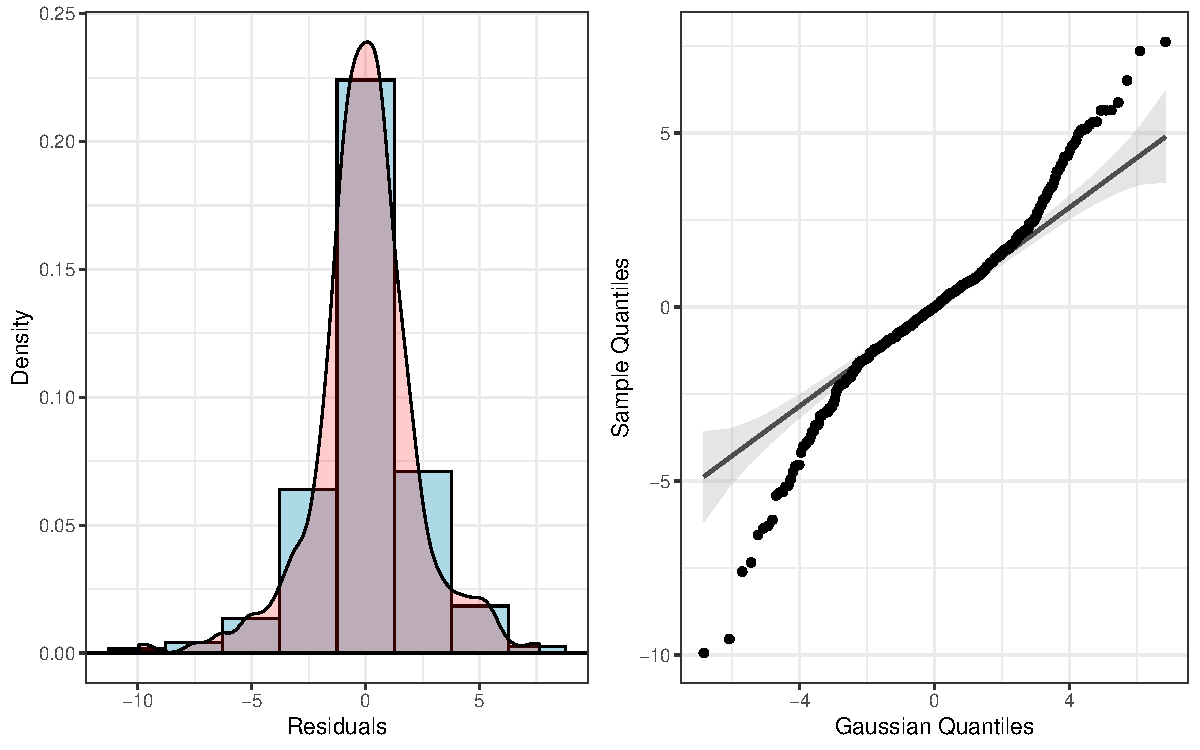
\includegraphics{HW4-022}

\begin{Schunk}
\begin{Sinput}
> sum(x4y4.mod$residuals) #close to zero
\end{Sinput}
\begin{Soutput}
[1] -8.09422e-15
\end{Soutput}
\end{Schunk}

\begin{Schunk}
\begin{Sinput}
> #check constance - plot residuals against fitted values
> ggdat<-data.frame(residuals=x4y4.mod$residuals,
+                   fitted=x4y4.mod$fitted.values)
> ggplot(data=ggdat, aes(x=fitted, y=residuals))+
+   geom_point(shape=1) +
+   geom_hline(yintercept=0, linetype="dashed")+
+   theme_bw()+
+   xlab(bquote(hat(Y)))+
+   ylab("Residuals")
\end{Sinput}
\end{Schunk}
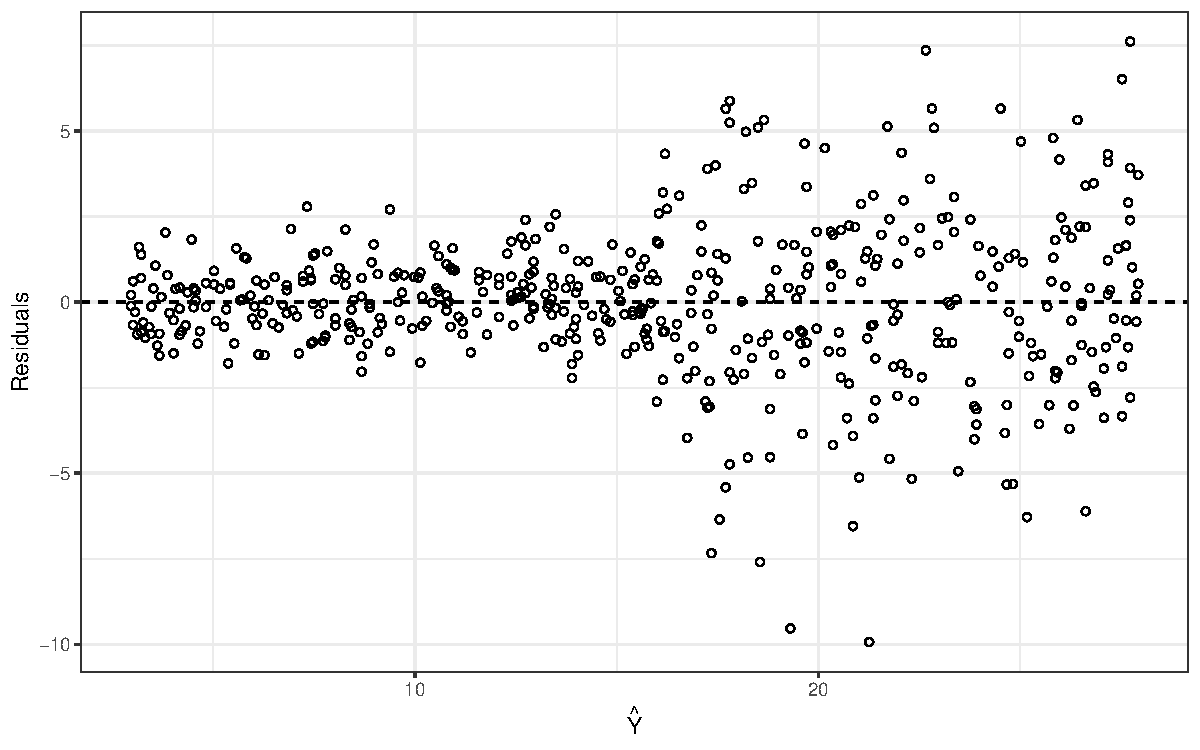
\includegraphics{HW4-024}
\end{enumerate}
%%%%%%%%%%%%%%%%%%%%%%%%%%%%%%%%%%%%%%%%%%%%%%%%%%%%%%%%%%%%%%%%%%%%%%%%%%%%%%%
%%%%%%%%%%%%%%%%%%%%%%%%%%%%%%%%%%%%%%%%%%%%%%%%%%%%%%%%%%%%%%%%%%%%%%%%%%%%%%%
%%%%%%%%%  Question 4
%%%%%%%%%%%%%%%%%%%%%%%%%%%%%%%%%%%%%%%%%%%%%%%%%%%%%%%%%%%%%%%%%%%%%%%%%%%%%%%
%%%%%%%%%%%%%%%%%%%%%%%%%%%%%%%%%%%%%%%%%%%%%%%%%%%%%%%%%%%%%%%%%%%%%%%%%%%%%%%
  \item Consider the following simulation. This looks intimidating, but it's
  a fairly simple exploration about what we'll talk about in class. This walks
  you through ``seeing" what's going on in the background.
  \begin{enumerate}
    \item Plot the data simulated below. Assess the linear relationship.
\begin{Schunk}
\begin{Sinput}
> set.seed(50)
> x_1<-sample(x=seq(0,100,0.01),size=50,replace=TRUE)
> e_1<-rnorm(n=50,mean=0,sd=5)
> y_1<-3.5+2.1*x_1 + e_1
\end{Sinput}
\end{Schunk}

\begin{Schunk}
\begin{Sinput}
> plot(x_1, y_1)
\end{Sinput}
\end{Schunk}
\begin{enumerate}
    \item Write out the population model.
    \begin{align*}
      Y_i &= \beta_0 + \beta_1 X_{1i} + \beta_2 X_{2i} + \epsilon 
    \end{align*}
    \item Fit the model based on the sample data and write out the sample model below.
    \item Add the regression line to the plot in black, with lwd=2 and lty=3.
    \item Check the assumptions of OLS for this model.
    \item Interpret the $R^2$ of the model.
    \item Interpret the overall $F$ test of the model. Report all 5 steps.
    \item Interpret the coefficients of the model; are they what you would expect?
\end{enumerate}
  \item Now, let's add a bad datapoint to the data created in part (a).
  \begin{enumerate}
    \item Plot the data simulated below; ensure to plot the  Assess the linear relationship.
\begin{Schunk}
\begin{Sinput}
> x_2<-c(x_1,100)
> y_2<-c(y_1,25)
\end{Sinput}
\end{Schunk}
    \item Fit the model based on the sample data and write out the sample model below.
    \item Check the assumptions of OLS for this model.
    \item Plot the data and regression lines from Questions 1-2. Add the regression line to the 
    plot in red.
    \item Interpret the coefficients of the model; are they what you would expect?
\end{enumerate}
  \item Continue with the data from Question b.
\begin{enumerate}
    \item Plot the residuals of your model against $x_2$ as well as the residuals 
    against predicted.
    \item Fit the appropriate model for estimating the weights for weighted least 
    squares regression.
    \item Provide a summary of the weights. How does the weight for the observation 
    (100,25) compare to the other observations?
    \item Use the weights from the previous part to fit a weighted least squares 
    regression.
    \item Check the assumptions of OLS for this model.
    \item Plot the data and regression lines from Questions 1-2. Add the regression 
    line to the plot in blue.
    \item Interpret the coefficients of the model; are they what you would expect?
  \end{enumerate}
  \item Continue with the data from parts (b,c).
  \begin{enumerate} 
    \item Fit a robust regression using Huber-weighted iterated reweighted least 
    squares and write out the sample model below.
    \item Plot the data and regression lines from Questions 1-3. Add the regression
    line to the plot in purple.
    \item Interpret the coefficients of the model; are they what you would expect?
  \end{enumerate}
  \item Continue with the data from parts (b,c,d).
  \begin{enumerate}
    \item Fit a robust regression using Bisquare-weighted iterated reweighted 
    least squares and write out the sample model below.
    \item Plot the data and regression lines from Questions 1-4. Add the regression 
    line to the plot in purple.
    \item Interpret the coefficients of the model; are they what you would expect?
  \end{enumerate}
  \item Continue with the data from parts (b,c,d,e).
\begin{enumerate}
    \item Fit a quantile regression and write out the sample model below.
    \item Plot the data and regression lines from Questions 1-5. Add the regression 
    line to the plot in black
    \item Interpret the coefficients of the model; are they what you would expect?
  \end{enumerate}
  \item Reflect on parts (a-f).
  \begin{enumerate}
    \item Which model is ``right"? If there's no one model 
      that is ``right", which one is ``best"?
    \item Rerun your code for Questions 1-6, but change the original sample size
    from 50 to 1000. There's no need to redo all of the parts from those questions,
    but discuss the difference. Look at the graph of the data with all the fitted
    regression models and compare it to that from the original data.
  \end{enumerate}
  \end{enumerate}
%%%%%%%%%%%%%%%%%%%%%%%%%%%%%%%%%%%%%%%%%%%%%%%%%%%%%%%%%%%%%%%%%%%%%%%%%%%%%%%
%%%%%%%%%%%%%%%%%%%%%%%%%%%%%%%%%%%%%%%%%%%%%%%%%%%%%%%%%%%%%%%%%%%%%%%%%%%%%%%
%%%%%%%%%  Question 5
%%%%%%%%%%%%%%%%%%%%%%%%%%%%%%%%%%%%%%%%%%%%%%%%%%%%%%%%%%%%%%%%%%%%%%%%%%%%%%%
%%%%%%%%%%%%%%%%%%%%%%%%%%%%%%%%%%%%%%%%%%%%%%%%%%%%%%%%%%%%%%%%%%%%%%%%%%%%%%%  
    \item \textbf{Case Study} The MASS package in \texttt{R} \citep{MASS} provides data about housing values
  in the Suburbs of Boston. The data provided is described below.
  \begin{itemize}
    \item \textbf{crim} -- per capita crime rate by town.
    \item \textbf{zn} -- proportion of residential land zoned for lots over 25,000 sq.ft.
    \item \textbf{indus} -- proportion of non-retail business acres per town.
    \item \textbf{chas} -- Charles River dummy variable (= 1 if tract bounds river; 0 otherwise).
    \item \textbf{nox} -- nitrogen oxides concentration (parts per 10 million).
    \item \textbf{rm} -- average number of rooms per dwelling.
    \item \textbf{age} -- proportion of owner-occupied units built prior to 1940.
    \item \textbf{dis} -- weighted mean of distances to five Boston employment centres.
    \item \textbf{rad} -- index of accessibility to radial highways.
    \item \textbf{tax} -- full-value property-tax rate per \$10,000.
    \item \textbf{ptratio} -- pupil-teacher ratio by town.
    \item \textbf{black} -- $1000(Bk - 0.63)^2$ where $Bk$ is the proportion of blacks by town.
    \item \textbf{lstat} -- lower status of the population (percent).
    \item \textbf{medv} -- median value of owner-occupied homes in \$1000s.
  \end{itemize}
  You can load this data using
\begin{Schunk}
\begin{Sinput}
> #install.packages("MASS",repos = "http://cloud.r-project.org/")
> library(MASS)
> data(Boston)
\end{Sinput}
\end{Schunk}
  Use your tools to build a regression model that predicts the median value of owner-occupied homes
  in \$1000s based on the other variables in the data set.
  
\begin{Schunk}
\begin{Sinput}
> mod<-lm(formula = medv ~ crim +. , data = Boston)
> summary(mod)
\end{Sinput}
\begin{Soutput}
Call:
lm(formula = medv ~ crim + ., data = Boston)

Residuals:
    Min      1Q  Median      3Q     Max 
-15.595  -2.730  -0.518   1.777  26.199 

Coefficients:
              Estimate Std. Error t value Pr(>|t|)    
(Intercept)  3.646e+01  5.103e+00   7.144 3.28e-12 ***
crim        -1.080e-01  3.286e-02  -3.287 0.001087 ** 
zn           4.642e-02  1.373e-02   3.382 0.000778 ***
indus        2.056e-02  6.150e-02   0.334 0.738288    
chas         2.687e+00  8.616e-01   3.118 0.001925 ** 
nox         -1.777e+01  3.820e+00  -4.651 4.25e-06 ***
rm           3.810e+00  4.179e-01   9.116  < 2e-16 ***
age          6.922e-04  1.321e-02   0.052 0.958229    
dis         -1.476e+00  1.995e-01  -7.398 6.01e-13 ***
rad          3.060e-01  6.635e-02   4.613 5.07e-06 ***
tax         -1.233e-02  3.760e-03  -3.280 0.001112 ** 
ptratio     -9.527e-01  1.308e-01  -7.283 1.31e-12 ***
black        9.312e-03  2.686e-03   3.467 0.000573 ***
lstat       -5.248e-01  5.072e-02 -10.347  < 2e-16 ***
---
Signif. codes:  0 ‘***’ 0.001 ‘**’ 0.01 ‘*’ 0.05 ‘.’ 0.1 ‘ ’ 1

Residual standard error: 4.745 on 492 degrees of freedom
Multiple R-squared:  0.7406,	Adjusted R-squared:  0.7338 
F-statistic: 108.1 on 13 and 492 DF,  p-value: < 2.2e-16
\end{Soutput}
\end{Schunk}

\begin{Schunk}
\begin{Sinput}
> #remove statistically insignificant variables
> mod1<-lm(formula = medv ~ crim + zn + chas + nox + rm + dis + rad + tax + ptratio + black + lstat, data = Boston)
> summary(mod1)
\end{Sinput}
\begin{Soutput}
Call:
lm(formula = medv ~ crim + zn + chas + nox + rm + dis + rad + 
    tax + ptratio + black + lstat, data = Boston)

Residuals:
     Min       1Q   Median       3Q      Max 
-15.5984  -2.7386  -0.5046   1.7273  26.2373 

Coefficients:
              Estimate Std. Error t value Pr(>|t|)    
(Intercept)  36.341145   5.067492   7.171 2.73e-12 ***
crim         -0.108413   0.032779  -3.307 0.001010 ** 
zn            0.045845   0.013523   3.390 0.000754 ***
chas          2.718716   0.854240   3.183 0.001551 ** 
nox         -17.376023   3.535243  -4.915 1.21e-06 ***
rm            3.801579   0.406316   9.356  < 2e-16 ***
dis          -1.492711   0.185731  -8.037 6.84e-15 ***
rad           0.299608   0.063402   4.726 3.00e-06 ***
tax          -0.011778   0.003372  -3.493 0.000521 ***
ptratio      -0.946525   0.129066  -7.334 9.24e-13 ***
black         0.009291   0.002674   3.475 0.000557 ***
lstat        -0.522553   0.047424 -11.019  < 2e-16 ***
---
Signif. codes:  0 ‘***’ 0.001 ‘**’ 0.01 ‘*’ 0.05 ‘.’ 0.1 ‘ ’ 1

Residual standard error: 4.736 on 494 degrees of freedom
Multiple R-squared:  0.7406,	Adjusted R-squared:  0.7348 
F-statistic: 128.2 on 11 and 494 DF,  p-value: < 2.2e-16
\end{Soutput}
\begin{Sinput}
> summary(mod1)$r.squared
\end{Sinput}
\begin{Soutput}
[1] 0.7405823
\end{Soutput}
\end{Schunk}

%%%%%%%%%%%%%%%%%%%%%%%%%%%%%%%%%%%%%%%%%%%%%%%%%%%%%%%%%%%%%%%%%%%%%%%%%%%%%%%
%%%%%%%%%%%%%%%%%%%%%%%%%%%%%%%%%%%%%%%%%%%%%%%%%%%%%%%%%%%%%%%%%%%%%%%%%%%%%%%
%%%%%%%%%  END!
%%%%%%%%%%%%%%%%%%%%%%%%%%%%%%%%%%%%%%%%%%%%%%%%%%%%%%%%%%%%%%%%%%%%%%%%%%%%%%%
%%%%%%%%%%%%%%%%%%%%%%%%%%%%%%%%%%%%%%%%%%%%%%%%%%%%%%%%%%%%%%%%%%%%%%%%%%%%%%%
\end{enumerate}
\bibliography{bib}
\end{document}
